\section{Evaluation}
\label{Evaluation}

In the following, I will evaluate the outcome of my optimization work. Using experimental benchmark data, I will discuss the impact of the optimizations on the three algorithms and reason about the influence of anchor positions on each algorithm's performance. I will also try to debate the statistic significance of these benchmarks.

\subsection{Approach}
As mentioned in Section~\ref{benchmarking}, the following data has been collected using my custom-made \emph{benchlat} utility. For this final benchmark, the algorithms were executed 500 times each, using 3, 4, and 5 anchors for AML and VBLE-OPT, and only 3 anchors in the case of Geo3, which simply discards additional anchors. The anchors were placed at random positions close to distinct borders of the playing area. For each set of anchors, the original implementation of each algorithm was executed as well in order to obtain a reference runtime. The achieved speed-up of each anchor/algorithm combination was calculated using Formula 1 shown below, where $t_{o,i}$ denotes the optimized runtime and $t_{r,i}$ is the reference runtime. The average speed-up was then derived using the usual formula for the arithmetic mean that is displayed in Formula 2.

\begin{align}
s_{i}& = \frac{t_{r,i}}{t_{o,i}} \\
\texttt{avg}(S)& = \frac{1}{n} \cdot \sum_{i = 1}^n s_{i}
\end{align}

The benchmarks were run on a quad-core Intel Xeon E31245 CPU with a clock frequency of 3.30 GHz, which had access to a total of 8 GB main memory. Because availability of this system was temporally limited, the number of algorithm iterations for each position needed to be reduced to 40, though, as execution runtimes are linearly dependent on the number of iterations, this does not compromise the significance of the benchmark results. The framework was configured to always use uniformly distributed errors. This, by contrast, limits the universality of the benchmark results to some degree. However, at the time of my coding it was the only error model implemented in LS$^{2}$.

\subsection{Discussion}
To begin with, all benchmark runs have delivered a positive result, i.e., the performance of each algorithm has been improved no matter where the anchors were placed. Table~\ref{average_table} shows the average speed-up calculated over all benchmark runs for each algorithm for 3, 4, and 5 anchors, providing a convenient overview of how much the algorithms benefitted from the optimization. AML boasts the best results with an average speed-up of 2.7 to 3.0, followed by Geolateration and VBLE-OPT.

\begin{table}[ht]
\begin{center}
\begin{tabular}{lccc} 
\toprule
& \multicolumn{3}{c}{Average speed-up} \\ 
\cmidrule(r){2-4}
Algorithm & 3 anchors & 4 anchors & 5 anchors \\
\midrule
AML & 2.70 & 2.91 & 3.01 \\
GEO3 & 2.20 & N/A & N/A \\ 
VBLE-OPT & 1.64 & 1.77& 1.75 \\
\bottomrule
\end{tabular}
\caption{Average speed-ups}
\label{average_table}
\end{center}
\end{table}

Most prominent here is the seemingly linear increase of the AML speed-ups, which was affirmed by (less numerous) experiments I conducted with 6 to 8 anchors. This is likely caused by the growing influence of the \emph{refinement} step, that could be perfectly vectorized due to the absence of conditional statements and thus has a considerable advantage over the scalar implementation. Using fewer anchors, the \emph{first intersection} step becomes the prevalent factor limiting the overall performance. However, as mentioned in the introduction, the theoretical speed-up of a SSE-based optimization is the number of vector elements, which is 4. I therefore suspect this increase to slowly decline with additive anchors until the speed-up factor has reached its peak, where it will probably stagnate.

In general, it is arguable whether these average speed-ups can be used to evaluate the success of my optimization work. The algorithms showed remarkable differences in the distribution of the test data, which can be seen in the box-and-whisker diagram in Figure~\ref{fig:boxplot}. Whereas speed-ups of AML and VBLE-OPT have a small variance, Geolateration has a considerably larger dispersion with its interquartile range spreading from around 2.05 to 2.35. I expect this to a be consequence of the many early-out conditionals contained in Geo3, which in general lead to huge variances in the algorithm runtimes. Some manual investigation into the anchor placements for speed-ups both from the lower and from the upper range of results suggested that input anchors forming a large triangle (e.g., anchors lying close to distinct corners of the playing area) led to higher speed-ups, whereas small, acute-angled triangles resulted in lower speed-ups. In the latter case, the optimizational step 4, which tests whether the minimum perimeter triangle is contained in the triangle formed by the anchors, is more likely to fail and therefore the remaining parts are executed more often. This also shows that the overall speed-up of Geo3 is not cumulative over the performance improvements of the various sections: Whereas the optimization of step 5, which calculates the geometric median of the final triangle, proved highly beneficial in my experiments, the overall speed-up of the optimization is higher in cases where it is executed less frequently (see also Figure~\ref{fig:scattergeo}).

In the case of Adapted Multilateration, the lower quartile is significantly larger than the upper quartile, with some outliers even outside the lower whisker range, which is set to $2.0 \cdot IQR$ (interquartile range). This may result from the \emph{first intersection} step

\begin{figure}
\begin{center}
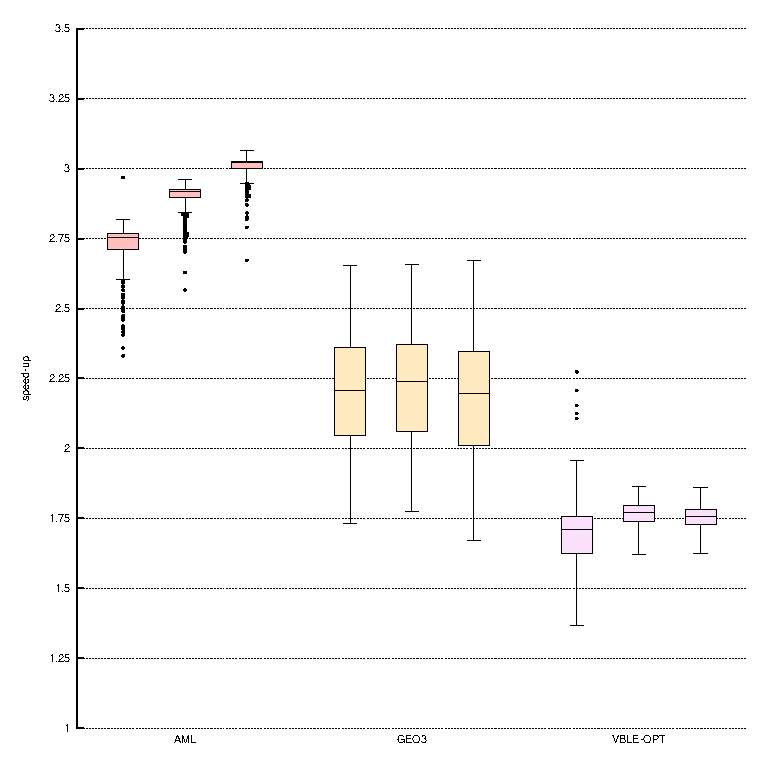
\includegraphics{img/boxplot}
\end{center}
\caption{Distribution of speed-ups}
\label{fig:boxplot}
\end{figure}

\begin{figure}
\begin{center}
\subfigure[AML (4 anchors)]{
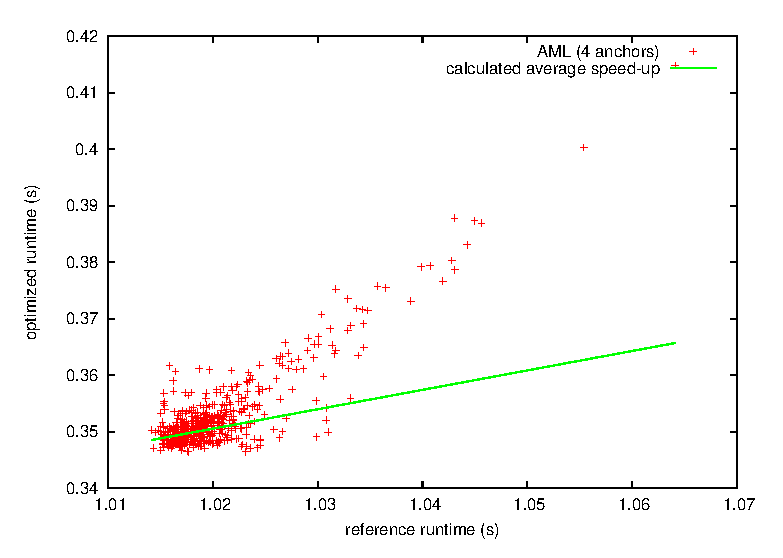
\includegraphics{img/scatter_aml4.eps}
\label{fig:scatteraml}
}
\subfigure[Geo3]{
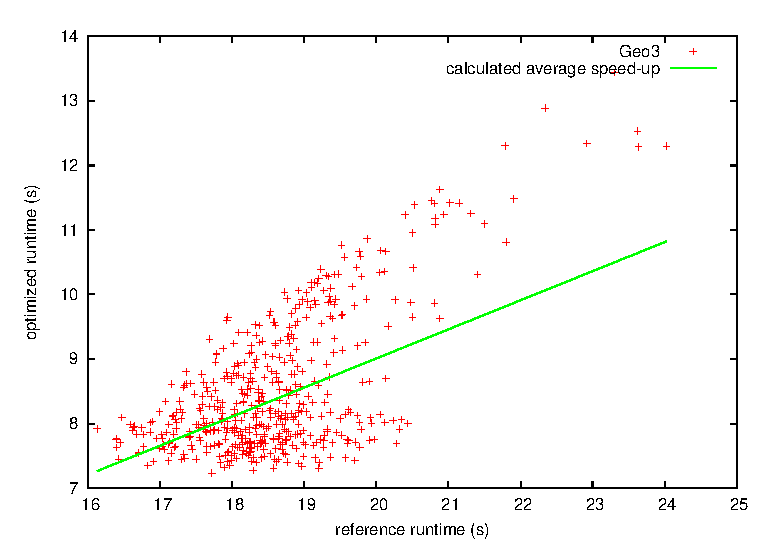
\includegraphics{img/scatter_geolat3.eps}
\label{fig:scattergeo}
}
%\subfigure[VBLE-OPT]{
%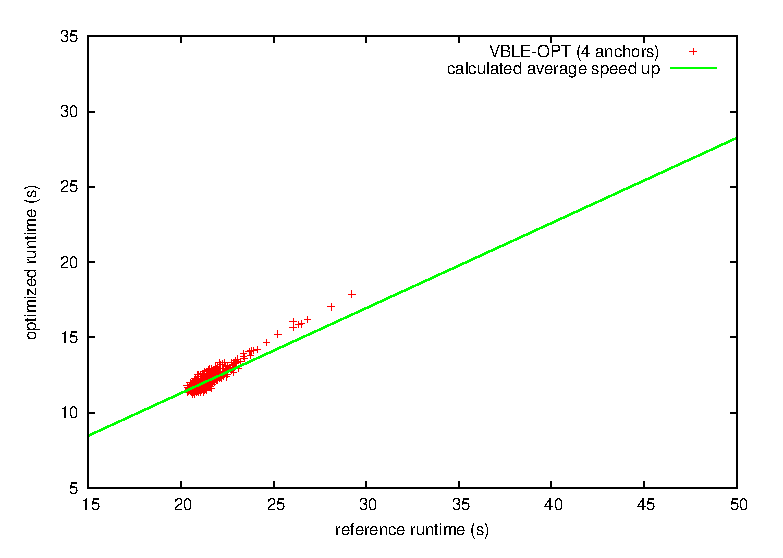
\includegraphics[width=0.3\textwidth]{img/scatter_vble4.eps}
%\label{fig:scattervble}
%}
\end{center}
\caption{Scatterplots of benchmark results}
\label{fig:scatterplots}
\end{figure}